\documentclass[11pt]{article}

\usepackage[margin=0.85in]{geometry}
\usepackage[T1]{fontenc}
\usepackage[utf8]{inputenc}
\usepackage{lmodern}
\usepackage{amsmath,amssymb,mathtools}
\usepackage{booktabs,longtable,array}
\usepackage{graphicx}
\usepackage{pdflscape}
\usepackage{microtype}
\usepackage{caption}
\usepackage{hyperref}

\hypersetup{
  colorlinks=true,
  allcolors=black,
  linkcolor=black,
  urlcolor=black,
  citecolor=black,
  pdftitle={Exact Lee--Yang Zeros, Self-Dual Susceptibility, and Lee--Yang Gap Scaling in Cylindrical Multilayer Solid-on-Solid Models}
}
\graphicspath{{./}}
\setlength{\emergencystretch}{2em}
\newcommand{\Z}{\mathbb{Z}}
\newcommand{\Ocal}{\mathcal{O}}
\newcommand{\R}{\mathbb{R}}
\newcommand{\tablevalue}[1]{\texttt{#1}}
\newcommand{\tableheading}[2]{\multicolumn{1}{>{\centering\arraybackslash}p{#1}}{#2}}

\title{Exact Lee--Yang Zeros, Self-Dual Susceptibility, and Lee--Yang Gap Scaling in Cylindrical Multilayer Solid-on-Solid Models}
\author{Wendel León Alvarado}
\date{November 12, 2026}

\begin{document}
\maketitle

\begin{abstract}
We connect cylindrical multilayer crown posets, monotone solid-on-solid (SOS) height configurations, and finite Lee--Yang partition functions. For the order polytope of $C_{k,n}$, its Ehrhart numerator $H_{k,n}(t)$ is the descent-generating polynomial of the linear extensions, so its coefficients are microcanonical excitation counts and $t$ is a grand-canonical fugacity. Exact certificates and Tensor-CRT contractions supply 23 palindromic polynomials for perimeters $3\le n\le7$, with all zeros isolated on the negative real axis and refined to 50 decimal digits. Reciprocal roots give a factorized quasiparticle representation of the free energy, excitation density, and susceptibility. Palindromicity proves the duality $\chi(1/t)=\chi(t)$; exact coefficient-positivity certificates further show that $t=1$ is the unique global susceptibility maximum in each of the 23 finite instances. For $n=3$, an exact two-mode recurrence proves that the thermodynamic free energy is analytic for every positive fugacity. We report finite-perimeter contraction ratios, compare the empirical zero distributions for $H_{8,3}$ and $H_{8,4}$ with their BKW phase densities, and provide reproducible vector and 300-dpi figures. The $n=4$ BKW curve is conditional on extending its observed order-three recurrence to all layer lengths.
\end{abstract}

\noindent\textbf{Keywords:} Lee--Yang zeros; order polytopes; P-partitions; solid-on-solid models; reciprocal polynomials; susceptibility; Beraha--Kahane--Weiss theory.

\section{Introduction and exact statistical-mechanical mapping}

Let $C_{k,n}$ be the cylindrical crown poset with vertices $x_{j,i}$, where $1\le j\le k$ is the layer and $i\in\Z/n\Z$ is the cyclic coordinate. Its cover relations are
\[
  x_{j,i}\prec x_{j+1,i},\qquad x_{j,i}\prec x_{j+1,i+1}
  \quad (1\le j<k).
\]
Write $d=kn$ for the number of vertices. The order polytope is
\[
  \Ocal(C_{k,n})=\{y\in[0,1]^d:y_u\le y_v\text{ whenever }u\preceq v\}.
\]
Its Ehrhart count and numerator are defined by
\begin{equation}
  L_{k,n}(m)=|m\Ocal(C_{k,n})\cap\Z^d|,
  \qquad
  \sum_{m\ge0}L_{k,n}(m)z^m=\frac{H_{k,n}(z)}{(1-z)^{d+1}}.
  \label{eq:ehrhart}
\end{equation}
Thus $L_{k,n}(m)$ is exactly the number of integer SOS height configurations
\[
  h_{j,i}\in\{0,1,\ldots,m\},\qquad
  h_{j,i}\le h_{j+1,i},\quad h_{j,i}\le h_{j+1,i+1},
  \label{eq:height-constraints}
\]
on the directed cylindrical cover graph. This is a monotone RSOS model with a hard height cap: $m$ is a microcanonical cutoff, and $L_{k,n}(m)$ is its exact configuration count. The inequalities are the full interaction; no nearest-neighbor constraint is added across the circumference beyond the displayed cyclic covers.

Label the vertices naturally by $n(j-1)+i+1$. The P-partition decomposition of order-preserving maps then gives
\begin{equation}
  H_{k,n}(t)=\sum_{\pi\in\mathcal{L}(C_{k,n})}t^{\operatorname{des}(\pi)}
  =\sum_{q=0}^{D}h_q^*t^q,
  \qquad D=d-k=k(n-1),
  \label{eq:partition}
\end{equation}
where $\mathcal{L}(C_{k,n})$ denotes the linear extensions and descents are measured in the natural labeling. Consequently $h_q^*$ is the microcanonical number of extension states with $q$ descent excitations, and
\[
  Z_{k,n}(t):=H_{k,n}(t)=\sum_{q=0}^{D}h_q^*t^q
\]
is their finite grand-canonical partition function. Its complex zeros are Lee--Yang zeros in the fugacity variable $t$ in the finite-system sense of Lee and Yang \cite{LeeYang1952}. This identification separates the height-cap count $L_{k,n}(m)$ from the excitation partition function $H_{k,n}(t)$; they are related by the Ehrhart generating function \eqref{eq:ehrhart}, but are not the same ensemble.

The crown posets are graded, and the corresponding $h^*$-polynomials are Gorenstein and palindromic:
\begin{equation}
  h_q^*=h_{D-q}^*,\qquad H_{k,n}(t)=t^D H_{k,n}(1/t).
  \label{eq:reciprocal}
\end{equation}
We use exact JSON certificates for the available cases with $n=3,4,5$ and $k\le8$. Tensor-CRT contractions reconstruct the additional numerators $H_{3,6}$, $H_{4,6}$, and $H_{3,7}$. The $n=4$ density comparison also requires $H_{8,4}$, which is reconstructed by the same exact method because no $C_{8,4}$ certificate file is present. In total, the study contains 23 polynomials. All roots were isolated using exact rational intervals for the reciprocal reduction and then refined with 75-digit mpmath arithmetic; the reported root values retain 50 significant decimal digits.

\section{Absence of a Positive-Fugacity Phase Transition for Narrow Cylinders}

For perimeter three, an exact transfer calculation proves for every $k\ge2$ the recurrence
\begin{equation}
  H_{k,3}(t)=P_3(t)H_{k-1,3}(t)+Q_3(t)H_{k-2,3}(t),
  \quad P_3(t)=t^2+6t+1,\quad Q_3(t)=t(t-1)^2,
  \label{eq:n3-recurrence}
\end{equation}
with $H_{0,3}=1$ and $H_{1,3}=t^2+4t+1$. The characteristic roots are
\begin{equation}
  \lambda_\pm(t)=\frac{P_3(t)\pm\sqrt{P_3(t)^2+4Q_3(t)}}{2}.
  \label{eq:n3-eigenvalues}
\end{equation}
For every real $t>0$, $P_3(t)>0$, $Q_3(t)\ge0$, and the discriminant is strictly positive. Hence $\lambda_+(t)>0$ is simple and strictly dominates $|\lambda_-(t)|$. The coefficient of $\lambda_+^k$ in the solution of \eqref{eq:n3-recurrence} is
\[
  A_+(t)=\frac{H_{1,3}(t)-\lambda_-(t)}{\lambda_+(t)-\lambda_-(t)}>0.
\]
It follows locally uniformly on $t>0$ that
\begin{equation}
  f_{\infty,3}(t):=\lim_{k\to\infty}\frac{1}{3k}\log H_{k,3}(t)
  =\frac13\log\lambda_+(t).
  \label{eq:free-energy-limit}
\end{equation}
The right-hand side is real analytic for every positive fugacity. Therefore the $n=3$ infinite-length model has no positive-real-fugacity thermodynamic singularity. This statement concerns the thermodynamic limit in layer length at fixed perimeter three; it does not rule out transitions in other limits where the perimeter also grows.

The same spectral analysis confines all finite $n=3$ zeros to
\begin{equation}
  I_3=(-7-4\sqrt3,-7+4\sqrt3)\subset(-\infty,0).
  \label{eq:i3}
\end{equation}
In particular, the positive fugacity axis is separated from the Lee--Yang zeros by a fixed interval around zero. The $n=3$ recurrence, confinement, and simple-root conclusion are exact for every $k\ge2$; the numerical table below is a finite sample of that theorem.

\section{Pitman quasiparticles and self-dual susceptibility}

For every studied instance, the zeros $r_1,\ldots,r_D$ are simple and strictly negative, and $H_{k,n}(0)=1$. Thus
\begin{equation}
  H_{k,n}(t)=\prod_{j=1}^{D}\left(1-\frac{t}{r_j}\right),
  \qquad
  p_j(t)=\frac{t}{t-r_j}.
  \label{eq:pitman-factorization}
\end{equation}
Each factor is the grand partition function of a two-state mode with occupation probability $p_j(t)$. The resulting independent-mode, or Pitman quasiparticle, representation yields
\begin{align}
  f_{k,n}(t)&=\frac{1}{kn}\log H_{k,n}(t),\\
  u_{k,n}(t)&=\frac{1}{kn}\sum_{j=1}^{D}p_j(t),\\
  \chi_{k,n}(t)&=\frac{1}{kn}\sum_{j=1}^{D}p_j(t)(1-p_j(t))
  =\frac{1}{kn}\sum_{j=1}^{D}\frac{-t r_j}{(t-r_j)^2}.
  \label{eq:thermodynamics}
\end{align}
Here $u$ is the excitation density and $\chi$ is its fugacity response (the specific-heat analogue in this dimensionless fugacity convention).

Reciprocity \eqref{eq:reciprocal} gives a direct duality. Let $U(t)=tH'_{k,n}(t)/H_{k,n}(t)=kn\,u_{k,n}(t)$. Differentiating the reciprocal identity gives
\[
  U(1/t)=D-U(t).
\]
Since $\chi(t)=tU'(t)/(kn)$, a second differentiation yields
\begin{equation}
  \chi_{k,n}(1/t)=\chi_{k,n}(t),
  \qquad
  u_{k,n}(1/t)=\frac{n-1}{n}-u_{k,n}(t).
  \label{eq:duality}
\end{equation}
The susceptibility is therefore stationary at the self-dual fugacity $t=1$. Palindromicity alone does not imply that this stationary point is a maximum. For the 23 exact polynomials considered here, we establish the stronger finite-instance result by an additional exact positivity certificate.

Set
\[
  N_{k,n}(t)=tH_{k,n}H'_{k,n}+t^2H_{k,n}H''_{k,n}-t^2(H'_{k,n})^2.
\]
Then $\chi_{k,n}(t)=N_{k,n}(t)/(knH_{k,n}(t)^2)$. Exact integer arithmetic for each of the 23 input polynomials gives
\begin{equation}
  N_{k,n}(1)H_{k,n}(t)^2-N_{k,n}(t)H_{k,n}(1)^2
  =(t-1)^2 C_{k,n}(t),
  \qquad C_{k,n}(t)\in\Z_{\ge0}[t]\setminus\{0\}.
  \label{eq:peak-certificate}
\end{equation}
The figure-generation script checks this coefficient condition directly from every exact coefficient vector. Since $H_{k,n}(t)>0$ for $t>0$, \eqref{eq:peak-certificate} proves $\chi_{k,n}(1)>\chi_{k,n}(t)$ for every $t>0$, $t\ne1$, in all 23 finite instances. Hence their unique global susceptibility peak is exactly
\begin{equation}
  t^*(k,n)=1.
  \label{eq:peak}
\end{equation}
This is a certified statement for the listed polynomials; no claim is made here that the coefficient-positivity certificate has been proved for every $k,n$.

\begin{figure}[htbp]
  \centering
  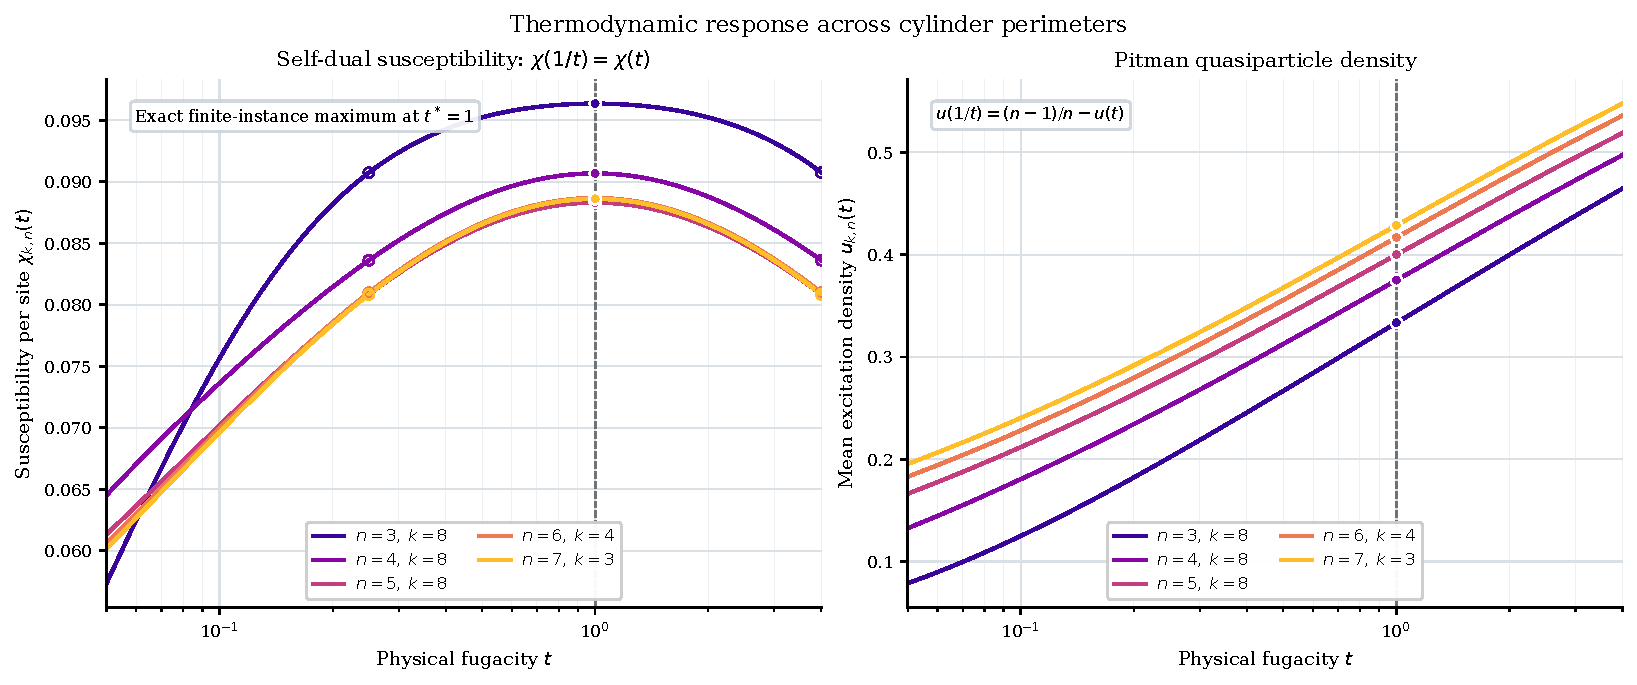
\includegraphics[width=0.97\linewidth]{fig_susceptibility_duality.pdf}
  \caption{Pitman excitation density and susceptibility for the largest available layer length at each perimeter: $k=8$ for $n=3,4,5$, $k=4$ for $n=6$, and $k=3$ for $n=7$. Curves are evaluated from the 50-digit root lists. The exact reciprocal relation is shown over $0.25\le t\le4$, and the center markers identify the certified global maximum $t^*=1$.}
  \label{fig:duality}
\end{figure}

\section{Finite-perimeter Lee--Yang gaps and BKW density}

Write $r_{\max}(k,n)$ for the negative zero closest to zero and $d_0(k,n)=|r_{\max}(k,n)|$. In the $n=3$ family, the exact edge in \eqref{eq:i3} implies
\[
  d_0(k,3)>7-4\sqrt3\quad(k\ge2).
\]
For the $n=4$ order-three recurrence studied in the source analysis, the BKW boundary is determined by
\[
  q_4(t)=t^4+76t^3-282t^2+76t+1,
  \quad z_0=-38-24\sqrt3,
  \quad \beta_+^{(4)}=\frac{z_0+\sqrt{z_0^2-4}}2,
\]
and the reported finite roots satisfy $d_0(k,4)>|\beta_+^{(4)}|$. Numerically, the two lower edges are $7-4\sqrt3\simeq0.07179677$ and $|\beta_+^{(4)}|\simeq0.01256966$. Figure~\ref{fig:gap} plots all available $d_0(k,n)$ values. Their perimeter means decrease from $0.08749$ at $n=3$ to $0.0005469$ at $n=7$. A descriptive exponential regression of those five means is $\bar d_0(n)\simeq3.013e^{-1.256n}$ with $R^2=0.991$; because the available $k$ ranges differ by perimeter, this finite-window fit is not an asymptotic law. The matched-$k$ contraction ratios also vary, from $0.1994$ between $n=3,4$ to $0.3094$ between $n=6,7$.

\begin{figure}[htbp]
  \centering
  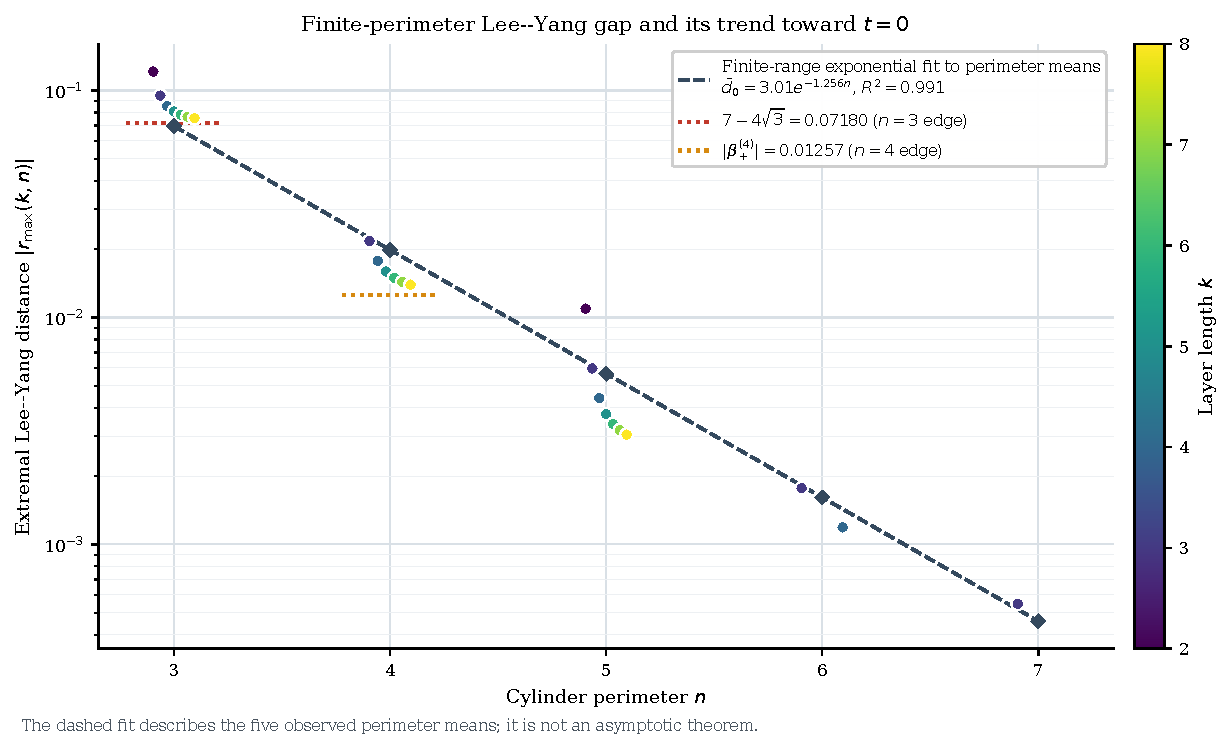
\includegraphics[width=0.94\linewidth]{fig_lee_yang_gap.pdf}
  \caption{Semilogarithmic Lee--Yang gap $d_0=|r_{\max}(k,n)|$ for all 23 instances, colored by layer length. Horizontal segments show the exact limiting lower edges for $n=3,4$. The dashed line fits the five perimeter means over the observed range only.}
  \label{fig:gap}
\end{figure}

Table~\ref{tab:instances} gives the finite-instance Lee--Yang and thermodynamic summary. Its extremal roots are rounded to 12 significant digits; the JSON file contains the full ordered root lists refined to 50 significant digits from exact rational Sturm isolating intervals. Here $D=k(n-1)$ is the polynomial degree, and the same file includes all 121-point thermodynamic grids.

\begin{landscape}
\tiny
\setlength{\tabcolsep}{2.3pt}
\renewcommand{\arraystretch}{1.22}
\begin{longtable}{@{}cc>{\raggedleft\arraybackslash}p{3.2cm}>{\raggedleft\arraybackslash}p{3.2cm}>{\raggedleft\arraybackslash}p{2.6cm}>{\raggedleft\arraybackslash}p{2.4cm}>{\centering\arraybackslash}p{1.0cm}>{\raggedleft\arraybackslash}p{2.6cm}@{}}
\caption{Finite-instance Lee--Yang and thermodynamic data. Extremal roots are rounded to 12 significant digits; full 50-digit lists are in the JSON file.}\label{tab:instances}\\
\toprule
\multicolumn{1}{c}{$k$} & \multicolumn{1}{c}{$n$} & \tableheading{3.2cm}{$r_{\min}$} & \tableheading{3.2cm}{$r_{\max}$} & \tableheading{2.6cm}{$d_0$} & \tableheading{2.4cm}{\shortstack{$\log_{10}$\\$(r_{\min}/r_{\max})$}} & \tableheading{1.0cm}{$t^*$} & \tableheading{2.6cm}{$\chi_{\max}$} \\
\midrule
\endfirsthead
\toprule
\multicolumn{1}{c}{$k$} & \multicolumn{1}{c}{$n$} & \tableheading{3.2cm}{$r_{\min}$} & \tableheading{3.2cm}{$r_{\max}$} & \tableheading{2.6cm}{$d_0$} & \tableheading{2.4cm}{\shortstack{$\log_{10}$\\$(r_{\min}/r_{\max})$}} & \tableheading{1.0cm}{$t^*$} & \tableheading{2.6cm}{$\chi_{\max}$} \\
\midrule
\endhead

2 & 3 & \tablevalue{-8.25108514330E+0} & \tablevalue{-1.21196179973E-1} & \tablevalue{1.21196179973E-1} & \tablevalue{1.83302213728E+0} & 1 & \tablevalue{1.04166666667E-1} \\
3 & 3 & \tablevalue{-1.05369769780E+1} & \tablevalue{-9.49038801251E-2} & \tablevalue{9.49038801251E-2} & \tablevalue{2.04543206234E+0} & 1 & \tablevalue{1.00694444444E-1} \\
4 & 3 & \tablevalue{-1.17161952468E+1} & \tablevalue{-8.53519405350E-2} & \tablevalue{8.53519405350E-2} & \tablevalue{2.13757320091E+0} & 1 & \tablevalue{9.89583333333E-2} \\
5 & 3 & \tablevalue{-1.23832885628E+1} & \tablevalue{-8.07539931681E-2} & \tablevalue{8.07539931681E-2} & \tablevalue{2.18567198646E+0} & 1 & \tablevalue{9.79166666667E-2} \\
6 & 3 & \tablevalue{-1.27923143686E+1} & \tablevalue{-7.81719375547E-2} & \tablevalue{7.81719375547E-2} & \tablevalue{2.21389824714E+0} & 1 & \tablevalue{9.72222222222E-2} \\
7 & 3 & \tablevalue{-1.30596050884E+1} & \tablevalue{-7.65719938110E-2} & \tablevalue{7.65719938110E-2} & \tablevalue{2.23186008886E+0} & 1 & \tablevalue{9.67261904762E-2} \\
8 & 3 & \tablevalue{-1.32432737360E+1} & \tablevalue{-7.55100302187E-2} & \tablevalue{7.55100302187E-2} & \tablevalue{2.24399071186E+0} & 1 & \tablevalue{9.63541666667E-2} \\
3 & 4 & \tablevalue{-4.60735733978E+1} & \tablevalue{-2.17044159212E-2} & \tablevalue{2.17044159212E-2} & \tablevalue{3.32690379359E+0} & 1 & \tablevalue{9.44865319865E-2} \\
4 & 4 & \tablevalue{-5.63395936570E+1} & \tablevalue{-1.77495067871E-2} & \tablevalue{1.77495067871E-2} & \tablevalue{3.50162742072E+0} & 1 & \tablevalue{9.29646880416E-2} \\
5 & 4 & \tablevalue{-6.27849422412E+1} & \tablevalue{-1.59273858397E-2} & \tablevalue{1.59273858397E-2} & \tablevalue{3.59571099812E+0} & 1 & \tablevalue{9.20495093666E-2} \\
6 & 4 & \tablevalue{-6.69691426589E+1} & \tablevalue{-1.49322502917E-2} & \tablevalue{1.49322502917E-2} & \tablevalue{3.65174947824E+0} & 1 & \tablevalue{9.14393185722E-2} \\
7 & 4 & \tablevalue{-6.98021797163E+1} & \tablevalue{-1.43262001855E-2} & \tablevalue{1.43262001855E-2} & \tablevalue{3.68773796914E+0} & 1 & \tablevalue{9.10034656703E-2} \\
8 & 4 & \tablevalue{-7.17946591975E+1} & \tablevalue{-1.39286126737E-2} & \tablevalue{1.39286126737E-2} & \tablevalue{3.71218427658E+0} & 1 & \tablevalue{9.06765759202E-2} \\
2 & 5 & \tablevalue{-9.14538399123E+1} & \tablevalue{-1.09344779941E-2} & \tablevalue{1.09344779941E-2} & \tablevalue{3.92240389021E+0} & 1 & \tablevalue{9.39516129032E-2} \\
3 & 5 & \tablevalue{-1.67913614690E+2} & \tablevalue{-5.95544323100E-3} & \tablevalue{5.95544323100E-3} & \tablevalue{4.45017182164E+0} & 1 & \tablevalue{9.15079365079E-2} \\
4 & 5 & \tablevalue{-2.26640334512E+2} & \tablevalue{-4.41227728574E-3} & \tablevalue{4.41227728574E-3} & \tablevalue{4.71067440503E+0} & 1 & \tablevalue{9.02341684294E-2} \\
5 & 5 & \tablevalue{-2.67051558472E+2} & \tablevalue{-3.74459525988E-3} & \tablevalue{3.74459525988E-3} & \tablevalue{4.85319023358E+0} & 1 & \tablevalue{8.94629147244E-2} \\
6 & 5 & \tablevalue{-2.94881532813E+2} & \tablevalue{-3.39119235600E-3} & \tablevalue{3.39119235600E-3} & \tablevalue{4.93929515074E+0} & 1 & \tablevalue{8.89480053470E-2} \\
7 & 5 & \tablevalue{-3.14418274510E+2} & \tablevalue{-3.18047671230E-3} & \tablevalue{3.18047671230E-3} & \tablevalue{4.99501556003E+0} & 1 & \tablevalue{8.85801388578E-2} \\
8 & 5 & \tablevalue{-3.28493654574E+2} & \tablevalue{-3.04419883329E-3} & \tablevalue{3.04419883329E-3} & \tablevalue{5.03305396965E+0} & 1 & \tablevalue{8.83042318189E-2} \\
3 & 6 & \tablevalue{-5.65745263491E+2} & \tablevalue{-1.76757997730E-3} & \tablevalue{1.76757997730E-3} & \tablevalue{5.50524185332E+0} & 1 & \tablevalue{8.97561710003E-2} \\
4 & 6 & \tablevalue{-8.41193092421E+2} & \tablevalue{-1.18878769810E-3} & \tablevalue{1.18878769810E-3} & \tablevalue{5.84979139551E+0} & 1 & \tablevalue{8.86748135954E-2} \\
3 & 7 & \tablevalue{-1.82862313954E+3} & \tablevalue{-5.46859535121E-4} & \tablevalue{5.46859535121E-4} & \tablevalue{6.52424842213E+0} & 1 & \tablevalue{8.86073318216E-2} \\
\endfoot
\end{longtable}
\end{landscape}

\subsection{BKW phase density and finite-size comparison}

For $n=3$, the dominant eigenvalues of \eqref{eq:n3-recurrence} form a conjugate pair on the negative interval $I_3$. If $\Psi_3(t)$ is the phase of the upper-half-plane eigenvalue, the limiting normalized density is
\begin{equation}
  \rho_3(t)=\frac{1}{3\pi}\left|\frac{d\Psi_3}{dt}\right|.
  \label{eq:bkw-density}
\end{equation}
For $n=4$, use the characteristic cubic
\[
  \lambda^3-P_4(t)\lambda^2-Q_4(t)\lambda-R_4(t),
\]
where
\[
  P_4=t^3+23t^2+23t+1,\quad
  Q_4=7t^5-28t^4-22t^3-28t^2+7t,\quad
  R_4=t(t-1)^6(t+1).
\]
On the BKW interval $I_4=(\beta_-^{(4)},\beta_+^{(4)})$, the phase $\Psi_4$ is the argument of the characteristic root with positive imaginary part, and $\rho_4(t)=|\Psi_4'(t)|/(4\pi)$. The $n=4$ expression is conditional: the order-three recurrence is verified for a finite initial range in the source work, while its validity for all $k$ is an explicit hypothesis of that BKW analysis. We therefore compare its phase density with the finite $H_{8,4}$ data without presenting it as an unconditional theorem for the entire Ehrhart sequence.

The empirical cumulative distribution is $N_{8,n}(t)/(8n)$, where $N_{8,n}(t)$ counts zeros up to $t$ in the corresponding negative interval. For $n=3$, the BKW and empirical total masses both equal $2/3$. For $n=4$, the grid-integrated BKW mass is $0.69212061$, whereas the finite $H_{8,4}$ empirical mass is $0.75$; the finite-size difference is retained rather than normalized away. The curve comparison, including the local finite-difference density, is in Fig.~\ref{fig:bkw}.

\begin{figure}[htbp]
  \centering
  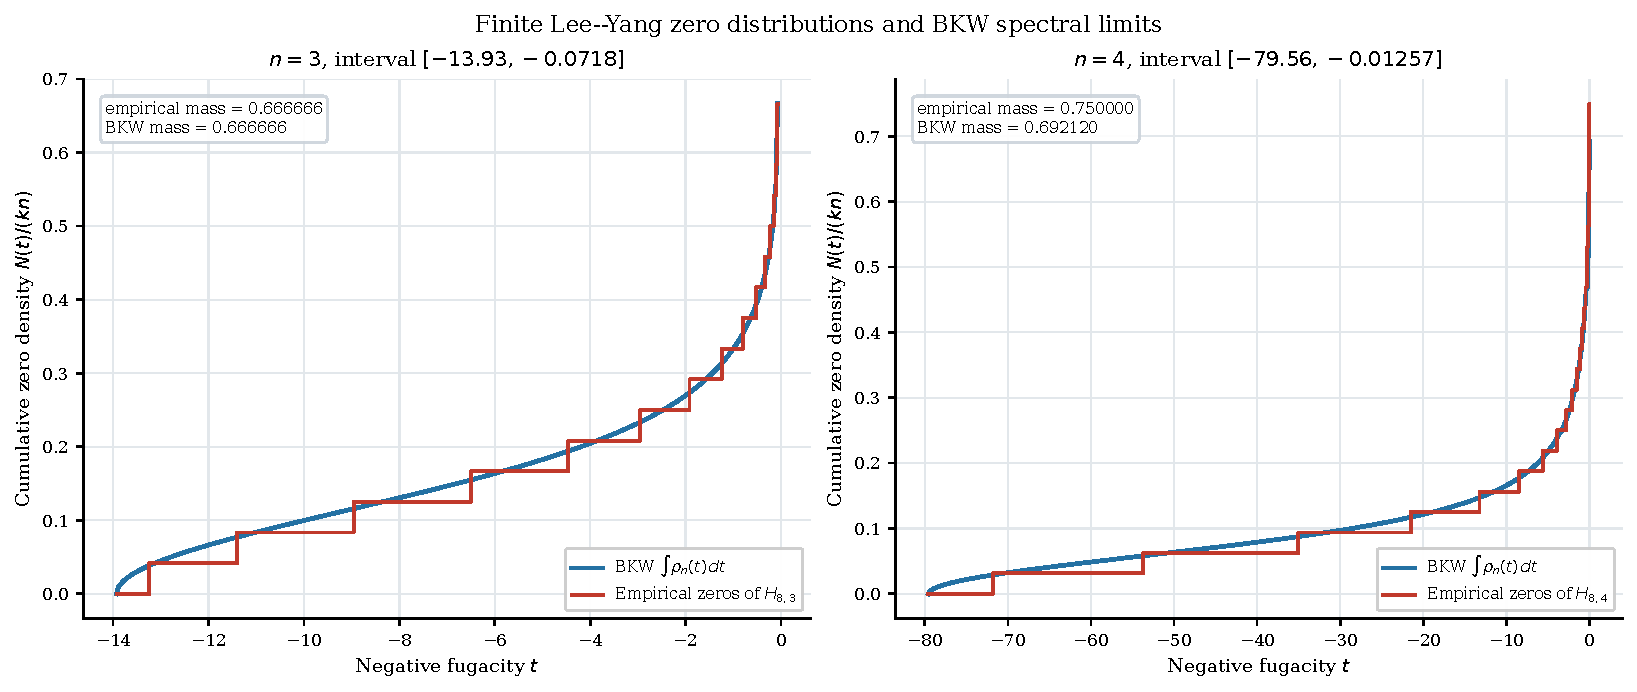
\includegraphics[width=0.97\linewidth]{fig_bkw_density.pdf}
  \caption{Empirical cumulative zero distributions of $H_{8,3}$ and $H_{8,4}$ against the integrals of their BKW phase densities. The $n=4$ limiting curve uses the conditional order-three recurrence and has smaller total mass than this finite sample.}
  \label{fig:bkw}
\end{figure}

\section{Conclusion and reproducibility}

The order-polytope/P-partition correspondence gives an exact statistical-mechanical interpretation of the cylindrical Ehrhart numerators. For $n=3$, an exact two-mode transfer proves analyticity of the positive-fugacity thermodynamic free energy. For the 23 finite instances, reciprocal roots yield the Pitman factorization, exact self-duality, and an exact coefficient certificate locating the unique susceptibility maximum at $t=1$. The extremal Lee--Yang distance contracts strongly across the observed perimeter range; the fitted exponential summarizes finite data and does not establish a uniform asymptotic law. The BKW comparison for $n=4$ remains conditional on the stated recurrence hypothesis.

All source code and numerical data are colocated in \texttt{LEE\_YANG\_PHYSICS/}. Reproduce the figures with \texttt{python generar\_graficas\_lee\_yang.py}; compile this manuscript twice with \texttt{pdflatex}. The analysis program \texttt{analyze\_lee\_yang\_physics.py} regenerates the exact polynomial, root, and thermodynamic JSON data.

\begin{thebibliography}{9}
\bibitem{LeeYang1952}
T. D. Lee and C. N. Yang,
Statistical theory of equations of state and phase transitions. II. Lattice gas and Ising model,
\emph{Physical Review} \textbf{87} (1952), 410--419.
\href{https://doi.org/10.1103/PhysRev.87.410}{doi:10.1103/PhysRev.87.410}.

\bibitem{Stanley1986}
R. P. Stanley,
Two poset polytopes,
\emph{Discrete \& Computational Geometry} \textbf{1} (1986), 9--23.
\href{https://doi.org/10.1007/BF02187680}{doi:10.1007/BF02187680}.

\bibitem{BKW1975}
S. Beraha, J. Kahane, and N. Weiss,
Limits of zeros of recursively defined polynomials,
\emph{Proceedings of the National Academy of Sciences} \textbf{72} (1975), 4209--4211.
\href{https://doi.org/10.1073/pnas.72.11.4209}{doi:10.1073/pnas.72.11.4209}.

\bibitem{BeckRobins}
M. Beck and S. Robins,
\emph{Computing the Continuous Discretely: Integer-Point Enumeration in Polyhedra},
2nd ed., Springer, 2015.
\end{thebibliography}

\end{document}
